\documentclass[10pt]{article}
\usepackage{NotesTeXV3,lipsum}
%\usepackage{showframe}

\begin{document}
\title{{NotesTeX}\\{\normalsize{\itshape{} An All\text{-}In\text{-}One Notes Package For Students}}}
\author{Aditya Dhumuntarao}
\affiliation{
	PhD. Student at the University of Minnesota\\
	\href{https://adhumunt.github.io/}{Website}\\
	\href{https://inspirehep.net/authors/1669979}{Inspire\text{-}HEP}\\
	\href{https://www.linkedin.com/in/aditya-dhumuntarao-80a0b8112/}{LinkedIn}\\ % chktex 8
	\href{https://github.com/Adhumunt}{GitHub}\\
}
\emailAdd{adhumunt@gmail.com}
\maketitle{}
\newpage{}
\pagestyle{fancynotes}
\part{Introduction}

\section{Required Packages}\label{sec:reqpackages}
\begin{margintable}\vspace{.8in}\footnotesize{}
	\begin{tabularx}{\marginparwidth}{|X}
		%Section~\ref{sec:motivation}. Motivation\\
		Section~\ref{sec:reqpackages}. Required Packages \\
		%Section~\ref{sec:license}. Margins\\
	\end{tabularx}
\end{margintable}
For \textit{NotesTeX,} the following packages are required
\begin{center}
	\texttt{marginnote, sidenotes, fancyhdr, titlesec, geometry, and tcolorbox.}
\end{center}
The role of each packages is discussed in Part~\ref{Part:Modification}. Briefly, the \texttt{marginnote}, \texttt{sidenote}, \texttt{titlesec}, and \texttt{tcolorbox} packages are required to create the \texttt{\( \backslash \)part} environment. \texttt{geometry} is used globally to set the page width, page height, and margin width. \texttt{fancyhdr} (overridden on the title, contents, and \texttt{\( \backslash \)part} page) sets the header.


\part{Modifications}\label{Part:Modification}
\section{Features}\label{sec:Features}
\begin{margintable}\vspace{1.4in}\footnotesize{}
	\begin{tabularx}{\marginparwidth}{|X}
		Section~\ref{sec:Features}. Features                 \\
		Section~\ref{sec:incpackage}. Included Packages      \\
		Section~\ref{Sec:Margins}. Margins                   \\
		Section~\ref{Sub:Special}. \texttt{amsthm} Environs. \\
		Section~\ref{sec:part}. Part Environment             \\
		Section~\ref{Sec: Fullpage}. Fullpage Environment    \\
	\end{tabularx}
	\caption{Contents for \textsc{Part II}}
\end{margintable}
\textit{NotesTeX} inherits \texttt{jhep} formatting for sections, subsections, subsubsections, title page, contents page, and bibliography presets. Significant extensions include the following:
\begin{enumerate}
	\item{} Several mathematics and physics packages.
	\item{} Margins and margin environments for tables, figures, and asides.
	\item{} \TeX\ shortcuts for various math scripts namely vector bold math such as \texttt{mathbb}, \texttt{mathfrak}, and \texttt{mathcal}.
	\item{} \texttt{amsthm} integrations and special environments for theorems, lemmas, proofs, definitions, examples, and remarks.\
	\item{} Stylized support for the \texttt{part} environment.
	\item{} A fullpage environment that spans across the text width and the margin for longer equations and horizontal figures.
\end{enumerate}
Each of these will be discussed in the following subsections.

\newpage{}
\section{Included Packages} % (fold)
\label{sec:incpackage}
Additional package are listed right under the required packages in \texttt{NotesTeX.sty}. These are divided into font styling packages and mathematical and physics related packages. The list of packages are also reiterated here and their links are in the sidenotes.
\begin{verbatim}
		\usepackage[T1]{fontenc}                            % Font Styling
		\usepackage{lmodern,mathrsfs}
	\end{verbatim}
\begin{margintable}\footnotesize{}
	\begin{tabularx}{\marginparwidth}{|X}
		\href{https://www.ctan.org/pkg/fontenc}{fontenc}     \\
		\href{https://www.ctan.org/pkg/mathrsfs}{mathrsfs}   \\
		\href{https://www.ctan.org/pkg/enumitem}{enumitem}   \\
		\href{https://www.ctan.org/pkg/mathtools}{mathtools} \\
		\href{https://www.ctan.org/pkg/amsfonts}{amsfonts}   \\
		\href{https://www.ctan.org/pkg/amsthm}{amsthm}       \\
		\href{https://www.ctan.org/pkg/bm}{bm}               \\
		\href{https://www.ctan.org/pkg/array}{array}         \\
		\href{https://www.ctan.org/pkg/tabularx}{tabularx}   \\
		\href{https://www.ctan.org/pkg/booktabs}{booktabs}   \\
		\href{https://www.ctan.org/pkg/graphicx}{graphicx}   \\
		\href{https://www.ctan.org/pkg/float}{float}         \\
		\href{https://www.ctan.org/pkg/caption}{caption}     \\
		\href{https://www.ctan.org/pkg/setspace}{setspace}   \\
		\href{https://www.ctan.org/pkg/multicol}{multicol}   \\
		\href{https://www.ctan.org/topic/pgf-tikz}{tikz}     \\ % chktex 8
		\href{https://www.ctan.org/pkg/physics}{physics}     \\
		\href{https://www.ctan.org/pkg/cancel}{cancel}
	\end{tabularx}
	\caption{Links}
\end{margintable}
\begin{verbatim}
		\usepackage[shortlabels]{enumitem}                  % Enumitem Options
		\usepackage{mathtools,amssymb,amsfonts,amsthm,bm}   % Math Presets
		\usepackage{array,tabularx,booktabs}                % Table Presets
		\usepackage{graphicx,wrapfig,float,caption}         % Figure Presets
		\usepackage{setspace,multicol}                      % Text Presets
		\usepackage{tikz,physics}                    % Physics Presets
	\end{verbatim}

% section prepackage (end)

\section{Margins}\label{Sec:Margins}%
\textit{NotesTeX} inherits all the margin commands that are used by \texttt{sidenote} and \texttt{marginnote}, and two additional pre\-configured commands known as \texttt{\( \backslash \)mn} and \texttt{\( \backslash \)sn}. The relevant commands, and the packages they belong to, are
\begin{center}
	\begin{multicols}{2}
		\noindent\texttt{
		\( \backslash \)marginnote~[marginnote]\\
		\( \backslash \)mn~[NotesTeX]\\
		\( \backslash \)sidenote~[sidenote]\\
		\( \backslash \)sn~[NotesTeX]\\
		\( \backslash \)lec~[NotesTeX]\\
		\( \backslash \)marginfigure~[sidenote]\\
		\( \backslash \)margintable~[sidenote]\\
		}
	\end{multicols}
\end{center}
The implementation of each of these is as follows.
\begin{enumerate}
	\item{} \texttt{Marginnote:} This is how a \texttt{\( \backslash \)marginnote\{\ldots{}\}} behaves.\marginnote{Not numbered, 10pt.}
	\item{} \texttt{Mn:} This is how a \texttt{\( \backslash \)mn\{\ldots{}\}} behaves.\mn{Numbered, footnotesize.}
	\item{} \texttt{Sidenote:} This is how a \texttt{\( \backslash \)sidenote\{\ldots{}\}} behaves.\sidenote{Numbered, 10pt.}
	\item{} \texttt{Sn:} This is how a \texttt{\( \backslash \)sn\{\ldots{}\}} behaves.\sn{Numbered, footnotesize.}
	\item{} \texttt{\textbackslash{} lec\textbraceleft{} Left Side\textbraceright\textbraceleft{} Some text goes here.\textbraceright} \texttt{Lec:} This environment appears in the left column and requires two inputs. The example here is \texttt{\textbackslash{} lec\textbraceleft{} Left Side\textbraceright\textbraceleft{} Some text goes here.\textbraceright}.\lec{Left Side}{Some text goes here.}
	\item{} \texttt{Marginfigure:} This environment requires the \texttt{\( \backslash \)begin\{marginfigure\}} {\( \cdots \)}\newline\texttt{\( \backslash \)end\{marginfigure\}} enclosings. The \texttt{caption} package is needed to caption the figure.
	\begin{marginfigure}
		\begin{center}
			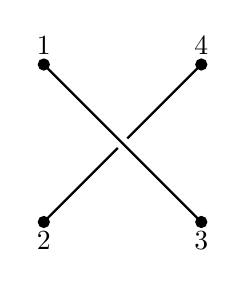
\begin{tikzpicture}
				\draw[black,thick] (-1,-1) -- (-.06,-.06); % chktex 8
				\draw[black,thick] (.06,.06) -- (1,1); % chktex 8
				\draw[black,thick] (-1,1) -- (1,-1); % chktex 8
				\filldraw[black] (-1,-1) circle (2pt) node[anchor=north] {2};
				\filldraw[black] (-1,1) circle (2pt) node[anchor=south] {1};
				\filldraw[black] (1,-1) circle (2pt) node[anchor=north] {3};
				\filldraw[black] (1,1) circle (2pt) node[anchor=south] {4};
			\end{tikzpicture}
		\end{center}
		\caption{Marginfigure: Tikz}
	\end{marginfigure}%
	\item{} \texttt{Margintable:} This environment requires the \texttt{\( \backslash \)begin\{margintable\}} {\( \cdots \)}\newline\texttt{\( \backslash \)end\{margintable\}} enclosings. A table package, such as \texttt{tabular}, \texttt{tabulary}, \texttt{tabu}, or \texttt{tabularx} is required. The \texttt{caption} package is needed to caption the table.
	\begin{margintable}
		\vspace{.1in}
		\begin{tabularx}{\marginparwidth}{|X|X|}
			\hline{}
			\textit{NotesTeX} & \textbf{rocks!} \\
			\hline{}
		\end{tabularx}
		\caption{Margintable}
	\end{margintable}	\end{enumerate}

\begin{remark}\textbf{Why use both \texttt{marginnotes} and \texttt{sidenotes}?}
	Quite simply, \texttt{marginnotes} overlap each other if they are too close whereas \texttt{sidenotes} both numbers and dynamically aligns all side notes, figures, and tables. However \texttt{sidenotes} cannot be used in equations, \texttt{multicols}, and with the \texttt{tcolorbox}\sn{See \ref{Sub:Special} and \ref{Sec: Fullpage} for more details.} environment. As the majority of the special environments from \texttt{amsthm} are modified to use \texttt{tcolorbox}, \texttt{marginnotes} becomes an essential part of \textit{NotesTeX}.
\end{remark}


\section{\texttt{amsthm} Environments}\label{Sub:Special}
\texttt{amsthm} environments are defined as usual being enclosed by \texttt{\( \backslash \)begin\{environment\}}\( \cdots \) \texttt{\( \backslash \)end\{environment\}}. Modifications include integration with the \texttt{tcolorbox} package. Note that counting for \texttt{theorems} and \texttt{lemmas} is distinct from the counting for \texttt{definitio} \texttt{ns}. Also, the \texttt{breakable} option for \texttt{tcolorbox} allows these environments to span multiple pages.

If one wishes to change the color, simply modify the line which states \texttt{borderline west=\{1pt\}}\texttt{\{0pt\}\textbraceleft{}blue\textbraceright{}}. The first numeric value dictates the width of the line, the second dictates how close it is away from the \textit{left} margin, while the last argument declares the color. This customization is independent of the \texttt{amsthm} environments.

There is one issue with this however. Since we are using a \texttt{tcolorbox}, this proof environment is incompatible with \texttt{\( \backslash \)sn} and \texttt{\( \backslash \)sidenote}, as it results in a \textbf{Float (s) Error}. However, this environment is compatible with \texttt{\( \backslash \)mn} and \texttt{\( \backslash \)marginnote}.

\begin{definition}
	The \texttt{definition} environment and the associated \texttt{tcolorbox} are provided by the following code in \texttt{NotesTeX.sty}:
	\begin{verbatim}
			\tcolorboxenvironment{definition}{
			  boxrule=0pt,
			  boxsep=0pt,
			  colback={White!90!Cerulean},
			  enhanced jigsaw, 
			  borderline west={2pt}{0pt}{Cerulean},
			  sharp corners,
			  before skip=10pt,
			  after skip=10pt,
			  breakable,
			}
		\end{verbatim}
\end{definition}
\begin{theorem}
	The \texttt{theorem} environment and the associated \texttt{tcolorbox} are provided by the following code in \texttt{NotesTeX.sty}:
	\begin{verbatim}
			\tcolorboxenvironment{theorem}{
			  boxrule=0pt,
			  boxsep=0pt,
			  colback={White!90!Dandelion},
			  enhanced jigsaw, 
			  borderline west={2pt}{0pt}{Dandelion},
			  sharp corners,
			  before skip=10pt,
			  after skip=10pt,
			  breakable,
			}
		\end{verbatim}
\end{theorem}
\begin{lemma}
	The \texttt{lemma} environment and the associated \texttt{tcolorbox} are provided by the following code in \texttt{NotesTeX.sty}:
	\begin{verbatim}
		\tcolorboxenvironment{lemma}{
		  boxrule=0pt,
		  boxsep=0pt,
		  blanker,
		  borderline west={2pt}{0pt}{Red},
		  before skip=10pt,
		  after skip=10pt,
		  sharp corners,
		  left=12pt,
		  right=12pt,
		  breakable,
		}
		\end{verbatim}
\end{lemma}
\begin{proof}
	The \texttt{proof} environment and the associated \texttt{tcolorbox} are provided by the following code in \texttt{NotesTeX.sty}:
	\begin{verbatim}
			\tcolorboxenvironment{proof}{
			  boxrule=0pt,
			  boxsep=0pt,
			  blanker,
			  borderline west={2pt}{0pt}{NavyBlue!80!white},
			  before skip=10pt,
			  after skip=10pt,
			  left=12pt,
			  right=12pt,
			  breakable,
			}
		\end{verbatim}
\end{proof}
\begin{example}
	The \texttt{example} environment and the associated \texttt{tcolorbox} are provided by the following code in \texttt{NotesTeX.sty}:
	\begin{verbatim}	
		\tcolorboxenvironment{example}{
		  boxrule=0pt,
		  boxsep=0pt,
		  blanker,
		  borderline west={2pt}{0pt}{Black},
		  sharp corners,
		  before skip=10pt,
		  after skip=10pt,
		  left=12pt,
		  right=12pt,
		  breakable,
		}
		\end{verbatim}
\end{example}
\begin{remark}
	The \texttt{remark} environment and the associated \texttt{tcolorbox} are provided by the following code in \texttt{NotesTeX.sty}:\mn{Coexistence of \texttt{amsthm} environment and \texttt{mn}}
	\begin{verbatim}
		\tcolorboxenvironment{remark}{
		  boxrule=0pt,
		  boxsep=0pt,
		  blanker,
		  borderline west={2pt}{0pt}{Green},
		  before skip=10pt,
		  after skip=10pt,
		  left=12pt,
		  right=12pt,
		  breakable,
		}
		\end{verbatim}
\end{remark}

\section{Fullpage Environment}\label{Sec: Fullpage}
\begin{fullpage}
	The \texttt{fullpage} environment is defined by
	\begin{center}
		\texttt{\( \backslash \)begin\{fullpage\}}\\
		\( \cdots \)\\
		\texttt{\( \backslash \)end\{fullpage\}}
	\end{center}
	with the width of the \texttt{fullpage} environment given by \texttt{\( \backslash \)textwidth}+\texttt{\( \backslash \)marginparsep}+\texttt{\( \backslash \)marginparwidth}.The code in \texttt{NotesTeX.sty} that is responsible for the \texttt{fullpage} environment is given by
	\begin{verbatim}
			\newenvironment{fullpage}{
			{\smallskip\noindent{}
			\begin{minipage}{\textwidth+\marginparwidth+\marginparsep}\hrule\smallskip\smallskip}
			{\smallskip\smallskip\hrule\end{minipage}\vspace{.1in}
			}
			}
			\end{verbatim}
\end{fullpage}
\begin{remark}
	Eliminating the \texttt{\( \backslash \)hrule} in the code will remove the lines surrounding the \texttt{fullpage} environment. Similarly, it is possible to change the vertical spacing after the \texttt{fullpage} is over, by modifying the \texttt{\( \backslash \)vspace\textbraceleft\textbraceright} argument.
\end{remark}

\begin{fullpage}
	\begin{multicols}{2}
		\texttt{multicols}\lec{lec}{entry}  may be used in conjunction with \texttt{fullpage}. I find it useful for formatting exercises in multiple columns and it makes the text distinct from the rest of the \texttt{fullpage} environment. The \texttt{lec} environment is compatible with \texttt{multicols} but \texttt{sidenote}, \texttt{marginnote} are not.\\

		%\lipsum[1]
	\end{multicols}
\end{fullpage}

\subsection{Known Issues with Fullpage}\label{Sub: Fullpage_Issues}
\begin{remark}
	Since the \texttt{fullpage} environment uses a \texttt{minipage}, and minipages do not work over multiple pages, one will need a new \texttt{fullpage} per page.
\end{remark}
\begin{remark}
	If the \texttt{twoside} option is enabled in the \texttt{documentclass} header, then the \texttt{fullpage} is known to bleed out beyond the margin.
\end{remark}

\section{The Part Environment}\label{sec:part}
In the original Jhep format, the \texttt{\( \backslash \)part} environment is not special and is set to the default given by the article class. In \textit{NotesTeX}, the \texttt{part} environment produces the following image. Furthermore the code responsible is noted below.\\
\begin{fullpage}
	{{\centering{}
				\begin{tcolorbox}[width=\marginparwidth,height=\marginparwidth/2,colback=black!50!white,colframe=black!50!white,center title,fonttitle=\bfseries\normalsize,title=PART,text fill]
					\begin{center}
						{\color{white}\Huge\bfseries\#}
					\end{center}
				\end{tcolorbox}
			}}
\end{fullpage}


\begin{fullpage}
	% {{\centering
	% 	\begin{tcolorbox}[width=\marginparwidth,height=\marginparwidth/2,colback=black!50!white,colframe=black!50!white,center title,fonttitle=\bfseries\normalsize,title=PART,text fill]
	% 	  \begin{center}
	% 	  {\color{white}\Huge\bfseries\#}
	% 	  \end{center}
	% 	\end{tcolorbox}
	% }}
	% ~ \newline 
	\begin{verbatim}
		\titleformat{\part}[hang]{{\thispagestyle{plain}}\Huge\bfseries}{\marginnote{
			\begin{tcolorbox}
			[width=\marginparwidth,height=\marginparwidth/2,colback=black!75!white,
			   colframe=black!75!white,center title,fonttitle=\bfseries\normalsize,title=PART,
			   text fill]

			  \begin{center}
			  	{\color{white}\thepart}
			  \end{center}

			\end{tcolorbox}
		}[-1.25in]}{0pt}{\Huge\bfseries}
	\end{verbatim}
\end{fullpage}

This combines the \texttt{titlesec} and the \texttt{tcolorbox} packages, placing the title of the \texttt{\( \backslash \)part} on the left hand side, and the \texttt{\( \backslash \)part} number in the margin.


\part{Advanced}
For those wanting to adjust the margin sizes, or the \texttt{fancyhdr} layout, there are a few comments that could be made here.
\section{Page Dimensions}
\textit{NotesTeX} relies on the \texttt{geometry} package to set its dimensions. The associated code is the deceptively simple chunk of code given by
\begin{verbatim}
		\geometry{paperheight=11in,paperwidth=8.5in,
          marginparsep=.02\paperwidth,marginparwidth=.2\paperwidth,
          inner=.11\paperwidth,voffset=-1in,headheight=.02\paperheight,
          headsep=.03\paperheight,footskip=20pt,
          textheight=.795\paperheight,textwidth=.62\paperwidth}
	\end{verbatim}
Ignoring most of the arguments, the \texttt{\( \backslash \)paperheight} and \texttt{\( \backslash \)paperwidth} are set to be the standard \(8.5\times11\) inches. All other options, with the exception of \texttt{\( \backslash \)voffset}, inherit fractions of \texttt{\( \backslash \)paperheight} and \texttt{\( \backslash \)paperwidth}, the most important being \texttt{\( \backslash \)marginparwidth}. Increasing \texttt{\( \backslash \)marginparwidth} causes the margin to bleed off of the right side of the page. In order to increase this value, \texttt{\( \backslash \)textwidth} must be decreased accordingly.


\section{\texttt{Fancyhdr} Layout}
As mentioned before, \texttt{fancyhdr} is overridden on the title page, the contents page, and the \texttt{\( \backslash \)part} page, and sets the header for all other pages through the code
\begin{verbatim}
	\pagestyle{fancy}%
	\newlength{\offset}%
	\setlength{\offset}{\marginparwidth{} + \marginparsep}%
	\renewcommand{\sectionmark}[1]{\markboth{#1}{}}%
	\renewcommand{\subsectionmark}[1]{\markright{#1}{}}%

	\fancypagestyle{fancynotes}{%
	  \fancyhf{}%
	  \fancyheadoffset[rh]{\offset}%
	  \renewcommand{\headrulewidth}{0pt}%
	  \fancyhead[L]{\textsc{\leftmark}}%
	  \fancyhead[R]{\footnotesize{} \textit{\rightmark}\quad\quad{} \thepage}%
	}%
	\end{verbatim}
The header style is set so that it spans the width of the entire page as opposed to just the \texttt{\( \backslash \)textwidth} through the line \texttt{\( \backslash \)fancyheadoffset[rh]\textbraceleft\( \backslash \)myoddoffset\textbraceright}. The \texttt{\( \backslash \)sectionmark} and \texttt{\( \backslash \)subsectionmark} are set up so that the \texttt{section} appears on the left and \texttt{subsections} appear on the right along with the page number, and this is given in the last two lines of code.


\section{Alternative Language Integration}
For languages written right to left, such as Persian, it is possible to use \textit{NotesTeX}. A complied example can be found in the legacy V1 version on Github. Suggestions are welcome for a more comprehensive language integration.

\section{License}\label{sec:license}
Aditya Dhumuntarao does not own the copyright to the original package, \texttt{jheppub.sty}. All modification have been approved by the Jhep Editorial committee, and permission has been attributed to Aditya to distribute freely the modified version of \texttt{jheppub.sty}, known as \texttt{NotesTeX.sty}.

This work may be distributed and/or modified under the conditions of the LaTeX Project Public License, either version 1.3 of this license or (at your option) any later version. The latest version of this license is found \href{http://www.latex-project.org/lppl.txt}{here}, and version 1.3 or later is part of all distributions of LaTeX version 2005/12/01 or later. The current maintainer of this work is Aditya Dhumuntarao.\footnote{Please contact me at my email if you have any questions or comments.} % chktex 8
\end{document}